\chapter{Analisi di algoritmi}

\section{Studio degli algoritmi}
Studiare gli algoritmi significa studiarne la \emph{complessità} e, l'obiettivo
di quest'analisi, è quello di realizzare nuove versioni di quegli stessi
algoritmi che godano di una \emph{complessità} minore e siano quindi più
efficienti.

\begin{definition}[Complessità di un algoritmo]
    Studiare la complessità di un algoritmo significa fare l'analisi delle risorse
    impiegate da un algoritmo per risolvere un problema, in funzione della
    dimensione e della tipologia di input.
\end{definition}\noindent
A questo punto la \emph{complessità} si misura con una funzione del tipo:
\[\text{Complessità}:\text{"Dimensione dell'input"}\rightarrow
\text{"Tempo di esecuzione"}\]
Ma cosa si intende con \emph{dimensione dell'input}?

\paragraph{Dimensione dell'input}
Ci sono due criteri per stimare la dimensione:
\begin{itemize}
    \item \emph{Criterio di costo uniforme}: la taglia dell’input è il numero
    di elementi di cui è costituito;
    \item \emph{Criterio di costo logaritmico}: la taglia dell’input è il
    numero di bit necessari per rappresentarlo;
\end{itemize}
E con \emph{tipologia di input}?
Questo aspetto non impatta su tutti gli algoritmi allo stesso modo. Il caso in
cui è più facile comprenderne le conseguenze è quello dell'ordinamento di array.
L'algoritmo \emph{insertion sort}, per esempio, si adatta più efficientemente
a situazioni in cui gli elementi vengono forniti uno per volta e l'algoritmo
\emph{selection sort} invece, è preferibile quando si hanno già tutti gli elementi
da ordinare\footnote{La complessità di questi algoritmi verrà discussa più nel
dettaglio nel corso di questo capitolo}.

\paragraph{Tempo di esecuzione}
Il \emph{tempo di esecuzione} coincide con il numero di istruzioni elementari.

\begin{definition}[Istruzione elementare]
    Un’istruzione si considera elementare se può essere eseguita
    in tempo "costante" dal processore.
\end{definition}

\newpage
\subsection{Modello di calcolo}
Nello studio degli algoritmi, un parametro da tenere in considerazione è il
\emph{modello di calcolo} utilizzato in quanto modelli diversi potrebbero
cambiare, in meglio o in peggio, la \emph{complessità} e l'efficienza di un
algoritmo.

\begin{definition}[Modello di calcolo]
    Un modello di calcolo è una rappresentazione astratta di un calcolatore.
\end{definition}\noindent
Analizziamo nel dettaglio questa definizione per capire quali caratteristiche
debba avere un \emph{modello di calcolo}:
\begin{itemize}
    \item \emph{Astrazione}: deve nascondere i dettagli tecnico-operativi;
    \item \emph{Realismo}: deve riflettere la situazione reale del sistema di
    calcolo;
    \item \emph{Potenza matematica}: deve consentire di trarre conclusioni
    \emph{formali} sul costo;
\end{itemize}
Esistono molteplici \emph{modelli di calcolo} e il modello della \emph{Macchina
di Turing} ne è un esempio. Tuttavia, nel corso della trattazione faremo
riferimento al \emph{Modello RAM}\footnote{\emph{RAM: Random Access Machine}}
caratterizzato da:
\begin{itemize}
    \item \emph{Memoria}: è costituita da infinite celle di dimensione finita
    \item \emph{Processore}: ha un set di istruzioni simili a quelli reali:
    \begin{itemize}
        \item Operazioni logico-aritmetiche;
        \item Istruzioni di controllo;
    \end{itemize}
    \item \emph{Costo uniforme}: il costo delle istruzioni elementari è
    uniforme;
\end{itemize}

\section{Studio di alcuni algoritmi}
Proviamo a vedere la logica dietro l'analisi della \emph{complessità} con degli
esempi.
\subsection{Minimo di un array}
Di seguito viene riportato l'algoritmo per l'estrazione del minimo elemento di
un array. La funzione prende in input un array di $n$ elementi e la relativa
dimensione $n$.

\begin{code}{Implementazione funzione min per la ricerca del minimo}
\begin{minipage}[t]{0.66\textwidth}
\ind\bc{ITEM} min(\bc{ITEM}[] A, \bc{int} n)\\
    \bc{ITEM} min = A[1]\\
    \indf for (i = 2 to n) do\\
        \indff if (A[i] < min) then\\
            min = A[i]\\
    \indf return min
\end{minipage}
\hfill
\begin{minipage}[t]{0.32\textwidth}
    $\begin{array}[t]{cc}
        \text{Costo} & \text{N. esecuzioni}\\
        c_1 & 1\\
        c_2 & n\\
        c_3 & n-1\\
        c_4 & n-1\\
        c5 & 1
    \end{array}$
\end{minipage}
\end{code}

\paragraph{Analisi del costo}
Analizziamo il costo di questo algoritmo. Ogni operazione elementare ha un tempo
costante di esecuzione che indicheremo con $c_i$ e ogni istruzione viene eseguita
un certo numero di volte.

\newpage\noindent
Indichiamo con $T(n)$ la \emph{funzione di costo} dell'algoritmo,
ovvero la funzione che ne traccia il tempo di esecuzione. Calcoliamo $T(n)$
sommando il tempo di esecuzione di ogni istruzione considerando anche il numero
di volte che ogni istruzione viene eseguita.
\[T(n)\begin{array}[t]{cl}
    = & c_1+c_2n+c_3(n-1)+c_4(n-1)+c_5\\
    = & (c_2+c_3+c_4)n+(c_1+c_5-c_3-c_4)\\
    = & an+b
\end{array}\]

\subsection{Ricerca binaria ricorsiva}
Consideriamo l'algoritmo per la ricerca binaria.
\begin{code}{Implementazione funzione binarySearch per la ricerca binaria}
\begin{minipage}[t]{0.55\textwidth}
    \footnotesize
    \ind\bc{int} binarySearch(\bc{ITEM}[] A, \bc{ITEM} v, \bc{int} i, \bc{int} j)\\
    \indf if (i > j) then\\
        return 0\\
    \indf else\\
        \bc{int} m = $\lfloor$(i + j) / 2$\rfloor$\\
        \indff if (A[m] = v) then\\
            return m\\
        \indff else if (A[m] < v) then\\
            return binarySearch(A, v, m + 1, j)\\
        \indff else\\
            return binarySearch(A, v, i, m - 1)\\
\end{minipage}
\hfill
\begin{minipage}[t]{0.43\textwidth}
    \footnotesize
    $\begin{array}[t]{ccc}
        \text{Costo} & \text{N. }(i>j) & \text{N. }(i\leq j)\\
        c_1 & 1 & 1\\
        c_2 & 1 & 0\\
        \\
        c_3 & 0 & 1\\
        c_4 & 0 & 1\\
        c_5 & 0 & 0\\
        c_6 & 0 & 1\\
        c_7+T(\lfloor(n-1)/2)\rfloor & 0 & 0/1\\
        \\
        c_7+T(\lfloor n/2\rfloor) & 0 & 1/0
    \end{array}$
\end{minipage}
\end{code}\noindent
La funzione prende in input un array $A$ ordinato in senso crescente, l'elemento
$v$ da cercare e due indici $i$ e $j$ che indicano rispettivamente l'estremo
destro e sinistro della porzione di array all'interno della quale ricercare
l'elemento\footnote{All'inizio indicano rispettivamente l'indice del primo e
dell'ultimo elemento}.

Nell'algoritmo sono presenti delle selezioni, che "modificano" il costo in
termini di tempo dell'algoritmo. Viene selezione un elemento \q{centrale}
nell'array e, se non è l'elemento cercato, si applica ricorsivamente l'algoritmo
alla parte di sinistra, se l'elemento cercato è minore di quello analizzato,
oppure alla parte destra. Per questa caratteristica dell'algoritmo si ha che la
parte di sinistra ha dimensione $(n-1)/2$, mentre quella di destra $n/2$.

\bigskip\noindent
Analizziamo il caso pessimo, cioè quello in cui l'elemento cercato non è presente
e quindi viene controllato l'intero array. Scegliamo di agire in questo modo così
da poter dare una stima del tempo massimo di esecuzione. Per lo stesso motivo,
ipotizziamo che l'elemento cercato sia maggiore di ogni elemento presente
nell'array e che quindi la chiamata ricorsiva venga effettuata sempre sulla parte
di destra che ha una dimensione maggiore.

Inoltre, per semplicità, assumiamo che l'array contenga un numero $2^k$ di
elementi e assegniamo ad ogni istruzione elementare un costo $c_i$.

\bigskip\noindent
Nella stima del costo dell'algoritmo abbiamo due casi:
\begin{itemize}
    \item $i > j$ per $n = 0$ quindi $T(n) = c_1 + c_2 = c$;
    \item $i\leq j$ per $n > 0$ quindi $T(n) = T(n/2)+c_1+\dots+c_7=
    T(n/2) + d$;
\end{itemize}
Possiamo vedere il tutto come una funzione che determina il costo dell'algoritmo:

\[T(n)=\begin{cases}
    T(n/2) & n\geq 1\\
    c & n = 0
\end{cases}\]
Poiché $T(n/2)$ rappresenta una chiamata ricorsiva, possiamo analizzare le varie
chiamate:
\[T(n)=\begin{array}[t]{cll}
    = & T(n/2)+d\\
    = & T(n/4)+2d\\
    = & T(n/8)+3d\\
    \dots\\
    = & T(1)+kd & n=2^k\Rightarrow k=\log n\\
    = & T(0)+(k+1)d\\
    = & kd+(c+d)\\
    = & d\log(n)+e
\end{array}\]

\subsection{Ordini di complessità}
Dall'analisi dei due algoritmi abbiamo ottenuto due espressioni matematiche:
$an+b$ e $d\log(n)+e$\footnote{Il logaritmo è sottinteso essere in base 2}.
Viste quelle espressioni, dette \emph{funzioni di complessità}, possiamo affermare
che i due algoritmi hanno rispettivamente un costo \emph{polinomiale} e
\emph{logaritmico}.

Queste due tipologie di costo sono anche dette \emph{ordini} o \emph{classi di
complessità} e la tabella sottostante ne riassume i principali.
\begin{table}[h]
    \centering
    \renewcommand{\arraystretch}{1.2}
    \begin{tabular}{|l|l|l|l|l|l|}
    \hline
    $\mathbf{f(n)}$ & $\mathbf{10^1}$ & $\mathbf{10^2}$ & $\mathbf{10^3}$ & $\mathbf{10^4}$ & \textbf{Tipo} \\ \hline
    $\log n$        & $3$             & $6$             & $9$             & $13$            & Logaritmico   \\ \hline
    $\sqrt{n}$      & $3$             & $10$            & $31$            & $100$           & Sublineare    \\ \hline
    $n$             & $10$            & $100$           & $1000$          & $10000$         & Lineare       \\ \hline
    $n\log n$       & $30$            & $664$           & $9965$          & $132877$        & Loglineare    \\ \hline
    $n^2$           & $10^2$          & $10^4$          & $10^6$          & $10^8$          & Quadratico    \\ \hline
    $n^3$           & $10^3$          & $10^6$          & $10^9$          & $10^{12}$       & Cubico        \\ \hline
    $2^n$           & $1024$          & $10^{30}$       & $10^{300}$      & $10^{3000}$     & Esponenziale  \\ \hline
    \end{tabular}
\end{table}

\section{Notazione asintotica}
Abbiamo quindi introdotto il concetto di \emph{ordine di complessità} come metro
di misura del costo di un algoritmo. Ora andremo ad introdurre uno strumento, la
\emph{notazione asintotica}, che ci permetterà di descrivere in maniera più
formale il costo di un algoritmo.

Quelle che andremo ad introdurre in realtà sono tre notazioni, indicate
rispettivamente dalle lettere $O$, $\Omega$, $\Theta$.

\begin{definition}[Notazione $O$]
    Sia $g(n)$ una funzione di costo. Si indica con $O(g(n))$ l'insieme delle
    funzioni $f(n)$ tali per cui:
    \[\exists\,c>0,\,\exists\,m\geq0:f(n)\leq c\cdot g(n)\quad\forall\,n\geq m\]
\end{definition}\noindent
Le funzioni $f(n)$ che rispettano questa disuguaglianza sono dette essere
\emph{$O$-grandi} di $g(n)$ e si scrive in simboli $f(n)=O(g(n))$. $g(n)$ è un
\emph{limite asintotico superiore} di $f(n)$, ciò significa che $f(n)$ cresce
al più come $g(n)$.\newpage

\begin{definition}[Notazione $\Omega$]
    Sia $g(n)$ una funzione di costo. Si indica con $\Omega(g(n))$ l'insieme
    delle funzioni $f(n)$ tali per cui:
    \[\exists\,c>0,\,\exists\,m\geq0:f(n)\geq c\cdot g(n)\quad\forall\,n\geq m\]
\end{definition}\noindent
Le funzioni $f(n)$ che rispettano questa disuguaglianza sono dette essere
\emph{$\Omega$-grandi} di $g(n)$ e si scrive in simboli $f(n)=\Omega(g(n))$.
$g(n)$ è un \emph{limite asintotico inferiore} di $f(n)$, ciò significa che $f(n)$
cresce almeno come $g(n)$.

\begin{definition}[Notazione $\Theta$]
    Sia $g(n)$ una funzione di costo, Si indica con $\Theta(g(n))$ l'insieme
    delle funzioni $f(n)$ tali per cui: 
    \[\exists\,c_1>0,\,\exists\,c_2>0,\,\exists\,m\geq0:
    c_1\cdot g(n)\leq f(n)\leq c_2\cdot g(n)\quad\forall\,n\geq m\]
\end{definition}\noindent
Le funzioni $f(n)$ che rispettano quella disuguaglianza sono dette essere
$\Theta$ di $g(n)$ e si scrive in simboli $f(n)=\Theta(g(n))$.
$f(n)$ è un $\Theta$ di $g(n)$, ovvero $f(n)=\Theta(g(n))$, se e solo se
$f(n)=O(g(n))$ e $f(n)=\Omega(g(n))$, da cui deriva che $f(n)=\Theta(g(n))$
significa che $f(n)$ cresce esattamente come $g(n)$.

\bigskip\noindent
Graficamente, se $f(n)=\Theta(g(n))$, si osserva un comportamento di questo tipo:

\begin{figure}[htbp]
    \centering
    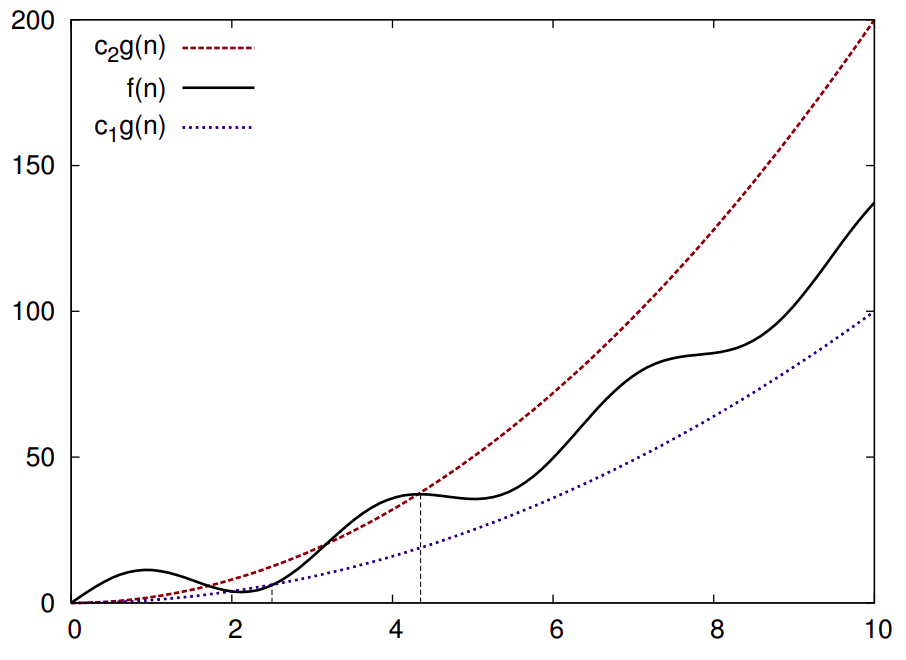
\includegraphics[width=\textwidth]{schema-theta.png}
    \caption{Curva di crescita di $f(n)=\Theta(g(n))$}
\end{figure}\noindent
Si noti come all'inizio la curva di $f(n)$ sembri disattendere le stime, ma
essendo \emph{stime asintotiche} esse valgono per $n\to+\infty$ e infatti,
superata una certa soglia, la curva di $f(n)$ rimane costantemente all'interno
della porzione di grafico disegnata dalle due curve di $g(n)$.

\begin{eg}[Verifica delle proprietà di un \bm{$O$}-grande]
    Si dimostri che $f(n)=10n^3+2n^2+7$ è un $O$-grande di
    $n^3$.

    \bigskip\noindent
    Riprendendo la definizione di \hyperref[def:4]{\emph{$O$}-grande}, dobbiamo
    dimostrare che:
    \[\exists\,c>0,\,\exists\,m\geq0:f(n)\leq c\cdot n^3\quad\forall\,n\geq m\]
    Procediamo:
    \[f(n)\begin{array}[t]{cll}
        =   &   10n^3+2n^2+7    & \\
        \leq&   10n^3+2n^3+7    & \qquad\forall\,n\geq1\\
        \leq&   10n^3+2n^3+n^3  & \qquad\forall\,n\geq\sqrt[3]{7}\\
        =   &   13n^3
    \end{array}\]
    A questo punto ci chiediamo se esistono un valore $c>0$ e un
    valore $m\geq 0$ tali che:
    \[13n^3\leq c\cdot n^3\]
    La risposta è banale poiché basta prendere $c\geq13$ e
    $m\geq1\geq\sqrt[3]{7}$, ad esempio, $m=2$.
\end{eg}
\begin{note}
    In questo esempio abbiamo potuto moltiplicare $2n^2$ per $n$
    e sostituire il $7$ con $n^3$, perché $n\geq0$. In realtà, nelle
    \emph{funzioni di costo} $n$ sarà sempre \emph{non negativo}, quindi lo
    potremo sempre fare.
\end{note}

\begin{eg}[Verifica delle proprietà di un \bm{$\Theta$}]
    Si dimostri che $f(n)=3n^2+7n$ è un $\Theta$ di $n^2$.

    \bigskip\noindent
    Procediamo verificando singolarmente i due estremi, inferiore e superiore.
    Iniziamo con lo studio del limite inferiore, cioè $\Omega$-grande. Ricordando
    la definizione di \hyperref[def:5]{\emph{$\Omega$}-grande} dobbiamo dimostrare
    che:
    \[\exists\,c_1>0,\,\exists\,m_1\geq0:f(n)\geq c_1\cdot n^2\quad\forall\,n\geq m_1\]
    Quindi:
    \[f(n)\begin{array}[t]{cll}
            =   &   3n^2+7n     & \\
            \geq&   3n^2        & \qquad\forall\,n\geq0\\
            \geq&   c_1\cdot n^2& \qquad\forall\,c_1\leq3\wedge\forall n\geq0
    \end{array}\]
    Pongo quindi $m_1=0$.

    \bigskip\noindent
    Passiamo ora allo studio del limite superiore. Come nell'esempio precedente
    dobbiamo dimostrare che:
    \[\exists\,c_2>0,\,\exists\,m_2\geq0:f(n)\leq c_2\cdot n^2\quad\forall\,n\geq m_2\]
    Quindi:
    \[f(n)\begin{array}[t]{cll}
        =   &   3n^2+7n     & \\
        \leq&   3n^2+7n^2   & \qquad\forall\,n\geq1\\
        =   &   10n^2       & \\
        \leq&   c_2\cdot n^2& \qquad\forall\,c_2\geq10\wedge\forall n\geq1
    \end{array}\]
    Pongo quindi $m_2=1$.

    \bigskip\noindent
    Torniamo ora al problema originario e riprendiamo la definizione di
    \hyperref[def:6]{$\Theta$}:
    \[\exists\,c_1>0,\,\exists\,c_2>0,\,\exists\,m\geq0:
    c_1\cdot g(n)\leq f(n)\leq c_2\cdot g(n)\quad\forall\,n\geq m\]
    Chiaramente, possiamo prendere $c_1=3$ e $c_2=10$, mentre,
    poiché l'ultima disequazione dev'essere vera $\forall\,n\geq m$,
    pongo $m=\max\{m_1,m_2\}=\max\{0,1\}=1$.

    \newpage\noindent
    Nel grafico seguente possiamo verificare la correttezza del
    nostri calcoli:
    \begin{figure}[h]
        \centering
        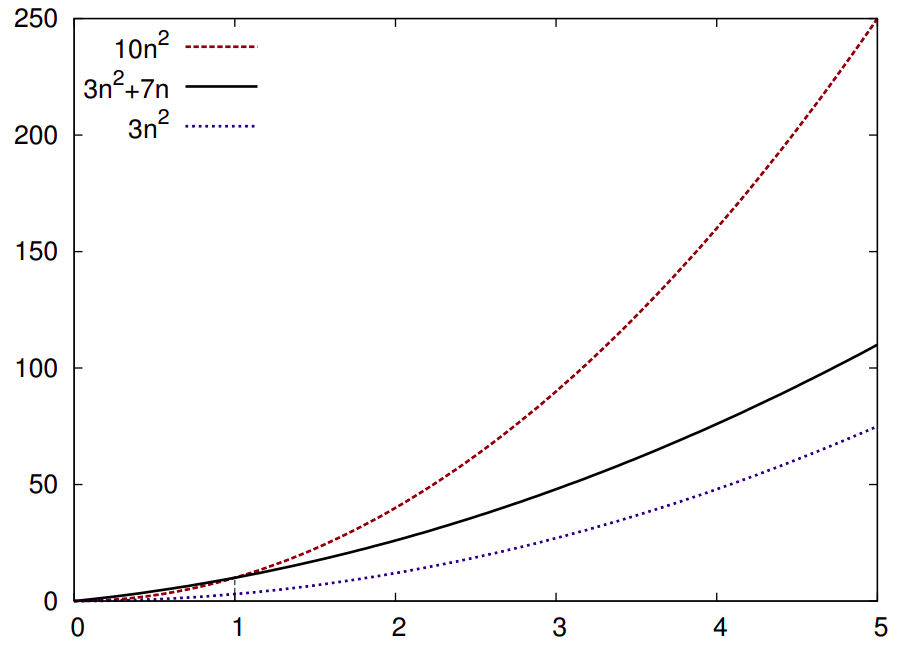
\includegraphics[scale=0.33]{schema-esempio-theta.png}
        \caption{Curva di $f(n)=3n^2+7n$}
    \end{figure}
\end{eg}

\section{Complessità degli algoritmi e dei problemi}
Solitamente, per risolvere uno stesso problema esistono una caterva di algoritmi
diversi e inevitabilmente alcuni sono più efficienti di altri. In che modo
lo studio della \emph{complessità} di questi \emph{algoritmi} può aiutarci a
capire la \emph{complessità del problema}?

Per rispondere a questa domanda sfruttiamo di nuovo la \emph{notazione
asintotica}.

\begin{definition}[Notazione $O$]
    Un problema ha complessità $O(f(n))$ se esiste almeno un algoritmo in grado
    di risolverlo che ha complessità $O(f(n))$.
\end{definition}

\begin{definition}[Notazione $\Omega$]
    Un problema ha complessità $\Omega(f(n))$ se tutti i possibili algoritmi che
    lo risolvono hanno complessità $\Omega(f(n))$.
\end{definition}

\paragraph{Notazione asintotica per gli algoritmi e per i problemi}
Nell'analisi della \emph{complessità degli algoritmi}, possiamo riassumere come
segue il significato delle \emph{notazioni asintotiche}:
\begin{itemize}
    \item $O(f(n))$: per tutti gli input $n$, l'algoritmo costa al più $f(n)$;
    \item $\Omega(f(n))$: per tutti gli input $n$, l'algoritmo costa almeno $f(n)$;
    \item $\Theta(f(n))$: per tutti gli input $n$, l'algoritmo costa $f(n)$;
\end{itemize}
Nell'analisi della \emph{complessità dei problemi}, vale invece:
\begin{itemize}
    \item $O(f(n))$: $O(f(n))$ è la complessità del miglior algoritmo in grado
    di risolvere il problema;
    \item $\Omega(f(n))$: vale se si riesce a dimostrare che nessun algoritmo
    può risolvere il problema in un tempo inferiore a $\Omega(f(n))$;
\end{itemize}
Se riusciamo a dimostrare che un problema ha complessità $O(f(n))$ e $\Omega(f(n))$,
un algoritmo con \emph{complessità} $\Theta(f(n))$ in grado di risolvere
quel problema, è il miglior algoritmo possibile.

\section[Ordinamento degli array in senso crescente]
{Ordinamento degli array in senso crescente\footnote{Il ragionamento è
analogo per ordinamenti in senso decrescente}}
Consideriamo ora tre diversi approcci al problema dell'ordinamento di array e
analizziamone la \emph{complessità}.

\subsection{Algoritmo Selection sort}
Questo algoritmo segue un approccio molto intuitivo: cerca il minimo tra tutti gli
elementi, lo ordina e poi ripete il tutto per i restanti elementi.

\begin{code}{Implementazione algoritmo Selection Sort}
\noindent\rmbreak SelectionSort(\bc{ITEM}[] A, \bc{int} n)\\
    \ind for (i = 1 to n - 1) do\\
        \indf\bc{int} min = min(A, i, n)\\
        \indf A[i] $\leftrightarrow$ A[min]\hfill\com{Scambia il minimo attuale e l'elemento $A[i]$}    
\end{code}
\vspace{-2\lineheight}
\begin{code}{Implementazione funzione min con indice di partenza arbitrario}
\noindent\rmbreak\ind\bc{int} min(\bc{ITEM}[] A, \bc{int} i, \bc{n})\\
    \bc{int} min = i\hfill\com{Posizione del minimo parziale}
    for (j = i + 1 to n) do\\
        \indf if (A[j] < A[min]) then\\
            \indff min = j\hfill\com{Nuovo minimo parziale}
    \ind return min
\end{code}\noindent
Quali sono le \emph{complessità} nei casi pessimo, medio e migliore?

\bigskip\noindent
Il caso pessimo è quello in cui l'array è ordinato in senso decrescente,
per cui ad ogni iterazione il minimo si trova nell'ultima posizione.
Il caso migliore è invece quello in cui l'array è già ordinato in senso crescente.
Nonostante questo, possiamo intuire che il costo dell'algoritmo non cambi, perché
in ogni caso si dovrà ricercare il minimo $n-1$ volte.

\bigskip\noindent
Provando a definire la \emph{funzione di costo} di questo algoritmo abbiamo:
\[\sum_{i=1}^{n-1}(n-i)=\sum_{i=1}^{n-1}i=\footnotemark\frac{n(n-1)}
{2}=n^2-\frac{n}{2}=O(n^2)\]
\footnotetext{\hyperlink{ser:1}{\emph{Formula di Gauss}}}
Questo vale per tutti i casi, quindi l'algoritmo \emph{insertion sort} ha un
costo $\Theta(n^2)$.

\subsection{Algoritmo Insertion sort}
Vediamo ora un approccio diverso al problema nel quale proviamo a prendere un
elemento per volta e a metterlo nella posizione giusta.

In particolare, ad ogni iterazione viene preso un valore e confrontato
progressivamente con i valori precedenti. Se viene trovato un valore minore di
quello preso, quest'ultimo viene salvato nella penultima cella
controllata.
\begin{code}{Implementazione algoritmo Insertion Sort}
\noindent\rmbreak\ind insertionSort(\bc{ITEM}[] A, \bc{int} n)\\
    for (i = 2 to n) do\\
        \indf \bc{ITEM} temp = A[i]\\
        \bc{int} j = i\\
        while (j > 1 and A[j - 1] > temp) do\\
            \indff A[j] = A[j - 1]\\
            j = j - 1\\
        \indf A[j] = temp
\end{code}\noindent
Cosa succede nei casi pessimo, medio e migliore?

\bigskip\noindent
Come prima, il caso pessimo è quello in cui l'array è ordinato in senso
contrario. In una situazione del genere, per ogni $i$ devono essere fatti $i-1$
confronti. Si ha quindi una funzione di questo tipo:
\[\sum_{i=2}^n(i-1)=\sum_{i=1}^{n-1}(n-i)=O(n^2)\]
Nel caso migliore invece, il vettore è già ordinato nel senso corretto col
risultato che ad ogni iterazione il controllo \texttt{A[j-1] > temp} è sempre
falso e quindi la funzione di costo è:
\[\sum_{i=2}^n1=n-2=O(n)\]

\hypertarget{sec:merge_sort}{\subsection{Algoritmo Merge sort}}
Questo algoritmo è basato sulla tecnica del \emph{divide-et-impera}, cioè procede
suddividendo l'array in due metà che vengono poi ordinate separatamente e quindi
ricombinate per ottenere l'array di partenza ordinato.

Come sarà facile intuire, questo algoritmo sfrutta la ricorsione per suddividere
l'array in due componenti e una qualche funzione per l'unione dei due sottoarray
ordinati.

\begin{code}{Implementazione algoritmo Merge sort}
\noindent\rmbreak\ind mergeSort(\bc{ITEM}[] A, \bc{int} first, \bc{int} last)\\
    if (first < last) then\\
        \indf\bc{int} mid = $\lfloor$(first + last) / 2$\rfloor$\\
        mergeSort(A, first, mid)\hfill\com{Ordina la parte sinistra}
        mergeSort(A, mid + 1, last)\hfill\com{Ordina la parte destra}
        merge(A, first, last, mid)\hfill\com{Combina i due sottoarray ordinati}
\end{code}\noindent
Nella funzione \texttt{merge} ipotizziamo di avere a disposizione un array di
appoggio $B$ nel quale andiamo ad inserire, in modo ordinato, i valori dei due
sottoarray di $A$. Una volta riempito, tutti i valori di $B$ vengono ricopiati
di nuovo su $A$.
\begin{code}{Implementazione funzione merge}
\noindent\rmbreak\ind merge(\bc{ITEM}[] A, \bc{int} first, \bc{int} last, \bc{int} mid)\\
    \bc{int} i, j, k, h\\
    i = first\\
    j = mid + 1\\
    k = first\hfill\com{Indice delle posizioni nell'array di appoggio}
    while (i $\leq$ mid and j $\leq$ last) do\hfill\com{Popolamento di $B$}
        \indf if (A[i] $\leq$ A[j]) then\\
            \indff B[k] = A[i]\\
            i = i + 1\\
        \indf else\\
            \indff B[k] = A[j]\\
            j = j + 1\\
        \indf k = k + 1\\
    \ind j = last\\
    for (h = mid downto i) do\\
        \indf A[j] = A[h]\\
        \indf j = j - 1\\
    \ind for (j = first to k - 1) do\hfill\com{Copia di $B$ su $A$}
        \indf A[j] = B[j]
\end{code}\noindent
Qual è la complessità del \emph{merge sort}?

\bigskip\noindent
Studiamo per prima la sola funzione \emph{merge}.
Nel ciclo \texttt{while} e nel secondo ciclo \texttt{for}, vengono fatte $n$
assegnazioni, dunque la funzione ha complessità $O(n)$.

Passando a considerare l'algoritmo nel suo insieme vediamo che l'array viene
diviso in due metà e poi viene invocata \emph{merge}. Ciò significa
che se si tracciano i partizionamenti dell'array durante l'esecuzione
dell'algoritmo, si ottiene un albero binario di altezza $k=\log n$\footnote{Per
semplicità ipotizziamo che il numero di elementi dell'array sia una potenza di 2}
nel quale, ad ogni livello $i$, la funzione $merge$ viene invocata $2^i$ volte.

\begin{figure}[hb]
\centering
\begin{tikzpicture}[node distance={20mm},main/.style={draw, circle, scale=0.95}]
	\node[main] (1) {$n$};

    \node[] (2) [below of=1] {$+$};
    \node[main] (3) [left of=2, xshift=-10mm] {$\frac{n}{2}$};
    \node[main] (4) [right of=2, xshift=10mm] {$\frac{n}{2}$};

    \node[] (5) [below of=3] {$+$};
    \node[main] (6) [left of=5, xshift=5mm] {$\frac{n}{2^2}$};
    \node[main] (7) [right of=5, xshift=-5mm] {$\frac{n}{2^2}$};

    \node[] (8) [below of=2] {$+$};

    \node[] (9) [below of=4] {$+$};
    \node[main] (10) [left of=9, xshift=5mm] {$\frac{n}{2^2}$};
    \node[main] (11) [right of=9, xshift=-5mm] {$\frac{n}{2^2}$};

    \node[] (12) [below of=6, xshift=-7.5mm] {$\vdots$};
    \node[] (13) [below of=6, xshift=7.5mm] {$\vdots$};

    \node[] (14) [below of=7, xshift=-7.5mm] {$\vdots$};
    \node[] (15) [below of=7, xshift=7.5mm] {$\vdots$};

    \node[] (16) [below of=10, xshift=-7.5mm] {$\vdots$};
    \node[] (17) [below of=10, xshift=7.5mm] {$\vdots$};

    \node[] (18) [below of=11, xshift=-7.5mm] {$\vdots$};
    \node[] (19) [below of=11, xshift=7.5mm] {$\vdots$};
    
    \node[] (20) [below of=12] {$+$};
    \node[main] (21) [below of=12, xshift=-7.5mm, yshift=-1mm] {$\frac{n}{2^k}$};
    \node[main] (22) [below of=12, xshift=7.5mm, yshift=-1mm] {$\frac{n}{2^k}$};

    \node[] (23) [below of=8] {};
    \node[] (24) [below of=23] {$\cdots$};

    \node[] (25) [below of=14] {$+$};
    \node[] (26) [below of=17] {$+$};

    \node[] (27) [below of=19] {$+$};
    \node[main] (28) [below of=19, xshift=-7.5mm, yshift=-1mm] {$\frac{n}{2^k}$};
    \node[main] (29) [below of=19, xshift=7.5mm, yshift=-1mm] {$\frac{n}{2^k}$};

    \node[] (30) [right of=29, xshift=7.5mm]
    {\hspace{0.8cm}\begin{tabular}{rl}
        $O(n)$ & $k=\log n$
    \end{tabular}};
    \node[] (31) [above of=30, yshift=-10mm] {$+$};
    \node[] (32) [above of=31, yshift=-10mm] {$\vdots$};
    \node[] (33) [above of=32, yshift=-10mm] {$+$};
    \node[] (34) [above of=33, yshift=-10mm]
    {\begin{tabular}{rl}
        $O(n)$ & $k=2$
    \end{tabular}};
    \node[] (35) [above of=34, yshift=-10mm] {$+$};
    \node[] (35) [above of=35, yshift=-10mm]
    {\begin{tabular}{rl}
        $O(n)$ & $k=1$
    \end{tabular}};
    \node[] (36) [above of=35, yshift=-10mm] {$+$};
    \node[] (37) [above of=36, yshift=-10mm]
    {\begin{tabular}{rl}
        $O(n)$ & $k=0$
    \end{tabular}};

    \draw (1) -- (3);
    \draw (1) -- (4);
    \draw (3) -- (6);
    \draw (3) -- (7);
    \draw (4) -- (10);
    \draw (4) -- (11);
    \draw (6) -- (12);
    \draw (6) -- (12);
    \draw (6) -- (13);
    \draw (7) -- (14);
    \draw (7) -- (15);
    \draw (10) -- (16);
    \draw (10) -- (17);
    \draw (11) -- (18);
    \draw (11) -- (19);
    \draw (12) -- (21);
    \draw (12) -- (22);
    \draw (19) -- (28);
    \draw (19) -- (29);
\end{tikzpicture}
\caption{Schema d'esecuzione del \emph{Merge sort}}
\end{figure}\noindent
Ogni livello ha un costo $O(n)$, quindi, essendoci $k=\log n$ livelli, il costo
dell'algoritmo è $O(n\log n)$. Possiamo verificare il nostro risultato
svolgendo direttamente i calcoli:
\[O\left(\sum_{i=0}^k2^i\cdot\frac{n}{2^i}\right)=O\left(\sum_{i=0}^kn\right)=
O(k\cdot n)=O(n\log n)\]
Nel primo passaggio, l'argomento della sommatoria è quello perché per ogni livello
sommiamo il costo necessario ad eseguire il merge su ogni sottoarray di dimensione
$\frac{n}{2^i}$ (e.g. il sottoarray al livello 1 avrà dimensione $\frac{n}{2^1}$),
ma consideriamo anche la numerosità dei sottoarray: $2^i$ per ogni livello $i$.

Ragionando anche sulla \emph{funzione di costo} constatiamo che, poiché ad ogni
livello vengono effettuate due invocazioni della \texttt{mergeSort} e
un'invocazione della \texttt{merge}, che ha costo $O(n)$, vale la seguente:
\[T(n)=\begin{cases}
    2T(n/2)+dn & n>1\\
    c & n=1\\
\end{cases}\]